\documentclass[12pt,oneside]{book}
\usepackage[english]{babel}
\usepackage[utf8]{inputenc}
\usepackage[T1]{fontenc}
\usepackage{helvet}
\usepackage{eso-pic,graphicx}
\usepackage[top=2cm, bottom=2cm, outer=1cm, inner=1cm]{geometry}
\usepackage{tikz}
\usetikzlibrary{positioning,shapes,shadows,arrows}
\usepackage{wrapfig}
\usepackage[most]{tcolorbox}

\newcommand{\showmap}[1]{
	\begin{center}
		\includegraphics[width=\linewidth]{#1}
	\end{center}
}

\newenvironment{blue-gem-list}{ 
    \begin{list}{
\includegraphics[scale=0.4]{images/blue-gem.png}}
    {}
}{
	\end{list}
}

\newtcolorbox{rpg-paperbox}[2][]{
		frame hidden,
		boxrule=0pt,
		breakable,
		enhanced,
		before skip=11pt plus 1pt,
		toptitle=3mm,
		boxsep=0.25ex,
		left=8pt,
		right=8pt,
		fonttitle=\fontfamily{fosj}\selectfont\scshape\bfseries\color{black},
		fontupper=\fontfamily{lmss}\selectfont,
		title=#2,
		arc=0mm,
		parbox = false,
		borderline north={1pt}{-0.5pt}{black},
		borderline south={1pt}{-0.5pt}{black},
		%colback=monstertandark,
		%colframe=monstertandark,
		%colbacktitle=monstertandark,
		fuzzy shadow={0mm}{-3.5pt}{-0.5pt}{0.4mm}{black!60!white},
		overlay={
			\fill [fill=black] (frame.south west) -- ++(7pt,0) -- ++(0,-5pt) -- cycle;
			\fill [fill=black] (frame.north west) -- ++(7pt,0) -- ++(0,5pt) -- cycle;
			\fill [fill=black] (frame.north east) -- ++(-7pt,0) -- ++(0,5pt) -- cycle;
			\fill [fill=black] (frame.south east) -- ++(-7pt,0) -- ++(0,-5pt) -- cycle;
		},
		after={\vspace{10pt plus 1pt}\noindent},
		#1
}



\begin{document}

\AddToShipoutPictureBG{
	
\includegraphics[width=\paperwidth,height=\paperheight]{images/vintage-vignette-tan-paper-texture-2}
}


\title{\textbf{Printii Apocalipsei}}
\maketitle

\pagenumbering{gobble}

\newpage

\tableofcontents

\newpage

\pagenumbering{arabic}

\chapter{Preambul}

\begin{quote}
A fost odata ca niciodata...\\
--Anonim
\end{quote}

\begin{rpg-paperbox}{Quest-ul Principal}
	O delegatie din Silvermoon catre Waterdeep s-a pierdut pe undeva prin zona si Lords Alliance vrea sa afle de ce si ce si cum si etc. 
\end{rpg-paperbox}
\\
Gheorghe, membru al Lords Alliance, a inceput sa investigheze ajutat de sensibila Ella Menstu si inteleptul Caesar.

Componenta echipei de delegati:
\begin{blue-gem-list}
	\item Teresiel - moon elf din Silverymoon
	\item Rhundorth - shield dwarf din Mirabar
	\item Deseyna Majarra - human noble din Waterdeep
\end{blue-gem-list}

Delegatia a fost vazuta ultima data la Beliard.

\newpage

\chapter{Jurnal}

\section{Inceputuri}

\begin{wrapfigure}{r}{0.25\textwidth}
    \centering
    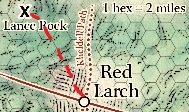
\includegraphics[width=0.25\textwidth]{images/maps/path-to-lance-rock}
\end{wrapfigure}

Suntem in Red Larch. Un oras nici prea mare, nici prea mic. Exact cat trebuie. 

Ne plimbam prin centru sa cautam masa si casa, ce mai e de cumparat, d-astea
turistice. Daca se poate mai ieftin ca na.

Nu gasim nimic ieftin dar tipa care detine o mina de piatra ne spune ca ar 
fi o comoara ascunsa intr-o pestera din apropiere. Mergem la pestera dar in 
loc de comoara gasim o armata de tantari. II ucidem si ne prindem ca aia
vroia sa faca o mina exploatare noua si nu putea din cauza tantarilor. 
Mergem la ea cu nervi si eventual ne da niste aur pentru serviciile prestate.

Nu prea mult dar suficient ca sa rezolvam cheltuielile curente cu cazarea 
si proviziile de drum.

Cum mai facem noi shopping prin oras un individ ne spune ca a vazut un 
craniu prins cu o sageta intr-un copac la Lance Rock. Hopa! 

Decidem sa investigam. 

Pe sageata infipta in copac gasim un pergament pe care scrie : \textit{``I will 
have the last laugh / You'll be next / Valklondar''}. Pergamentul e
facut din piele umana. Craniul pare sa fie in copac de cateva saptamani. In 
lipsa de idei lasam o nota cu o provocare. Ducem pielea la Tannery iar 
pielarul gaseste un tatuaj pe ea - un triunghi cu un trident deasupra.
\\
Cat timp am fost plecati o caverna aflata chiar sub piata centrala 
colapseaza. Ajutam un copchil cazut sa iasa si dupa aia ne bagam sa vedem 
care-i treaba. In dungeon gasim pumnalul \textit{Raszus} si un copil (altul), 
fiul lui Hatherhand. Tatal l-a trimis cu un mesaj important spre xyz. Aflam 
de Larak care i-a ajutat pe Believers (societatea secreta din sat) sa 
inteleaga semnele de la dweleri.

Eventual descoasem toata povestea si se pare ca Larak era un agent al cultul 
pamantului care folosea tot felul de trucuri ca sa-i pacaleasca pe sateni 
si sa-i recruteze.

Dupa ce se mai linistesc lucrurile prin sat mergem la crasma sa tragem 
una mica. Dupa mai multe mici Gheorghe aude o conversatie la o masa 
alatura, da cu pumnul in masa proprie si spune:
\textit{``Am auzit ca formatia pizdei aleia de m-a enervat (Windharrow) 
trebuie sa aiba o reprezentatie in Feathergale Spire  asa ca prima oara o 
sa ii fac o vizita.''}

\begin{wrapfigure}{l}{0.25\textwidth}
    \centering
    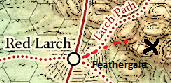
\includegraphics[width=0.25\textwidth]{images/maps/path-to-feathergale-spire}
\end{wrapfigure}

Zis si facut.

In Feathergale Spire stau Cavalerii Aerului, pasionati de calarit grifoni si de 
vanatoare. Se afla in in Sighing Valley, undeva la est de Red Larch.

Cand ajungem acolo gasim un turn inalt, dildonic, acoperit de marmura alba. 
In turn se poate intra printr-un drawbrige deschis peste o prapastie de 
400 de picioare. Mai e o intrare la baza turnului dar o ignoram.

Reusim sa intram pretizand ca suntem o formatie de trubaduri. Inauntru tragem
de limba pe cine putem.

\begin{rpg-paperbox}{Temple Of Howling Hatred}
Cica Windharrow lucreaza undercover si e de fapt mana dreapta
a printesei Aerului - Savra. Atm Windharrow s-a dus cu o misiune secreta 
in Temple Of Howling Hatred.
\end{rpg-paperbox}

\begin{rpg-paperbox}{Printesa Savra}
Printesa Savra este, la randul ei undercover, cavaler al aerului. A fugit 
din Waterdeep unde sunt multi inamici ai Cultului Aerului.
\end{rpg-paperbox}

Cultul aerului este in razboi cu cultul apei, pamantului si focului.

Ii ajutam pe cavaleri sa dea jos o manticora care tulbura ecosistemul din 
Sighing Valley si astfel le castigam increderea, o cina copioasa si 
cazarea peste noapte.

Gheorghe are un duel amical cu un cavaler si castiga. Ella se imbata. 
Caesar se furiseaza noaptea si fura ceva haur din camera lui Thurl.

\begin{rpg-paperbox}{Sacred Stone Monastery}
La plecare Thurl ne sugereaza sa investigam Sacred Stone Monastery. E mult
evil acolo cica.
\end{rpg-paperbox}

Revenim in Red Larch sa mai vindem , sa mai cumparam , arama-i veche, 
tabla-i veche. Localnicii sunt deja familiarizati cu noi si un pic 
mai sociabili. Cand ne plimbam de la un magazin la altul mai aflam 
tot felul de chestii de la tot felul de bagatori in seama.

\begin{rpg-paperbox}{Cartile Dwarfice}
Un individ shady din Wombford a facut rost de mai multe carti dwarfice. 
Cartea cumparata de Vallivoe din Red Larch contine istoria Waterdeep-ului 
si este veche de 500 de ani.
\end{rpg-paperbox}

De la un alt individ dubios cu caruta stricata si marcata cu un Castron
aflam de intalnirea druizilor la Scarlet Moon Hall.

Gheorghe isi ia armura noua si o poarta cu mandrie.Caesar sta trist in 
fata unui pahar de tarie in  care tot pune cuburi de gheata generate cu 
crituri de Frozen Arrow.

Ella plateste unui sexomancer de la han 100g si isi schimba sexul, numele 
si poza. Devine Axxl Menstu.

Dupa evenimentele din Feathergale decidem sa investigam disparitia diplomatilor 
la Beliard  via Scarlet Moon Hall. E in drum oricum. 

Cand ajungem stam de vorba cu niste druizi un pic betivani de la care aflam 
ca a-II-a zi urmeaza sa aiba loc un ritual al fertilitatii. Un ritual de 
sa fie bine sa nu fie rau. 

Urcam un pic pe deal si dam de o tabara mica cu cativa druizi unde-i priponit 
si un urs. Dupa un pic de conversatie despre vreme si taxe suntem atacati. 
Druizii sunt de fapt Flame Priests. Reusim sa-i batem.

Mai departe dam de o tabara cu doi tipi urat mirositori si anti-sociali. Nu 
reusim sa stabilim un raport social si continuam la a-IV-a tabara. Se repeta 
patania cu Flame Priest. Din fericire ne ajuta niste druizi ai izvorului apei 
limpezi care erau prin zona si cei doi tipi care de fapt sunt varcolaci. Cu 
greu reusim sa-i invingem. 

Deja cam oricine poarta gluga e suspect. Aparent, toti de pe deal au o agenda.

Ma rog, continuam la urmatoarea tabara unde dam de cativa ``druizi'' si de un 
tip pe nume Sauruki.  Se pare ca Sauruki e un cultist al apei. Ne invata fara 
sa vrea mudra cultului. Iarasi ne batem, iarasi castigam.

La tabara estica dam peste niste bugbears nespalati si niste druizi morti. 
Relativ repede, in tabara raman niste druizi morti si niste bugbears nespalati 
morti.

Ne intalnim cu \textbf{Lothar}, un cleric-fost-razboinic care a pornit pe 
calea spalarii pacatelor. Decide ca obiectivele lui coincid cu ale noastre 
si da join la party.

In sfarsit ajungem in varful dealului. Din niste corturi imprumutam cape 
de Moon Hall druids. Absolut accidental invocam un Flame Elemental din 
momaia care ardea molcom. Din motive care nu le stim dar suspectam ca 
au legatura cu imbracamintea, elementalul ne ignora si se duce la vale.
Luam xp gras desi nu meritam.

\begin{wrapfigure}{r}{0.25\textwidth}
    \centering
    
\includegraphics[width=0.25\textwidth]{images/dm-smiles}
\end{wrapfigure}

Cat incercam sa intelegem ce s-a intamplat apare o patrula. Un caine al 
focului ne miroase si ne luam wipe. In acest moment se intampla un 
reload. \textit{Doar} un caine ne miroase si reusim sa-l omoram. Mars 
sarla in focul care te-a nascut!

Ne urcam in turnul din varful dealului lasand cateva cadavre de garzi in 
urma. Mai aruncam cativa baieti de la inaltime si eventual ne intalnim cu 
\textit{Efizar}, seful local. Cu o incredere in sine deosebita si niste 
pretentii absurde ne oftica si ii dam. Din fericire are un lapsus si uita 
incantantia pentru Wall of Fire. Reusim sa-l luam prizonier si sa-l interogam.
Aflam despre niste diplomati care au fost ingropati la Shallow Graves si 
 despre intrarea secreta de la baza turnului in Fireland/Lumea Focului.

\section{2016-11-20}

De la Scarlet Moon Hall ne intoarcem in Red Larch. Cumparam
chestii. 

\begin{rpg-paperbox}{Shallow Graves}
	Larmon Greenboot, un cioban din sat, ne-a spus ca au aparut niste 
morminte noi cu cateva zile in urma pe unde paste el oile.
\end{rpg-paperbox}

\begin{blue-gem-list}
	\item mormantul 1: dwarf in haine de artizan, blacksmith
	\item mormantul 2: female human warrior, un simbol cu o secure rosie 
	(simbolul armatei din mirabar)
	\item mormantul 3: male human warrior, pelerina neagra si o armura din 
	piatra
	\item mormantul 4: male human, roba alba, pene negre pe umeri
\end{blue-gem-list}

Gasim un \textbf{tattered gray cloak} indiciu.

Continuam pe  drumul de la est si intr-o poienita gasim urmele unei batalii:
\begin{blue-gem-list}
	\item 2 morminte de piatra
	\item 8 bugbears cu armura neagra care au un simbol un triunghi
	\item 1 female human cu masca aurie sub forma unui gargoyle si roba are 
	un simbol un triunghi
	\item ne dam seama ca s-a folosit powerful earth magic
\end{blue-gem-list}

Luam \textbf{masca aurie} - indiciu.

Conform urmelor, un grup de 30 bugbears/oameni au plecat catre rau (vest). 
La rau sunt  urme de barci care au fost lansate la apa. Probabil toata escorta 
delegatilor a fost omorata aici.

Coboram la sud pe mal si gasim o tabara cu water priests si mercenari. Tragem
cu urechea si auzim ca seful water priests se numeste \textit{Jolliver Grimjaw}.
Ne batem si ii omoram.

Dupa ce ne sfatuim continuam cu barca spre Riverguard. E posibil ca atacatorii sa
fi mers acolo.

Rivergard are zidurile chiar pe malul raului. Se poate intra dinspre uscat via 
gatehouse sau pe apa printr-un port unde sunt ancorate niste barci.
Fortareata este in reparatie - acoperis nou. Un banner alb cu o manusa de 
armura (gauntlet) albastra.

Ajungem cu barca pe malul opus al raului, nevazuti. 

\section{2016-11-27}


In Riverguard Keep ne intamplina locotenentul Reashing care ne trimite la Jolliver.
Desi suntem calificati, Jolliver nu vrea sa ne angajeze ca mercenari si 
plecam  huiduind. 

Pare ca am pierdut interviul cand Axxel a pomenit de colaborarea 
artistica cu Windharrow.

Noaptea ne strecuram in  castel si incepem sa asasinam garzile cu dibacie. Caesar 
a renuntat la Frost Arrow cu succes.

Fragezim bine un Wave Priest si il facem prizonier. Aflam de la el ca sefii lui Jolliver sunt Greenjaw si Ushnara si ca vin din Templul Apei. Priest-ul nu ne poate spune nimic despre lupta din padure sau daca exista prizonieri.

\begin{rpg-paperbox}{Vaporul}
Gheorghe trage cu urechea la o camera de garda si aude ceva despre un vapor care
vine sau pleaca sau pleaca sau vine.
\end{rpg-paperbox}

\section{2016-12-04}

A progresat nitel asaltul asupra Riverguard Keep, Caesar si-a gasit un companion 
(temporar, sadly) si Gheorghe a inceput sa-si dea seama ca desi e util sa fii 
foarte scary in timpul interogatoriului, ajuta si sa pui intrebarile corecte.

Incet, incet progresam prin baraca, biserica si in sfarsit ajungem la corabia din 
port. Acolo o intalnim pe \textit{Shaolar Quanderil} care are pregatita o ambuscada.
Ambuscadorii mor. O interogam pe Shaolar si aflam ca atacul asupra delegatiei a fost 
facut de cultul pamantului. Cica si cultul apei pregatise ceva similar dar nu au reusit 
sa-si intinda capcana.

\begin{rpg-paperbox}{Temple of the Crashing Wave}
Ordinele au venit de la templul apei (Temple of the Crashing Wave), mai exact de la 
Gar Shatterkeel.
\end{rpg-paperbox}

Cultul apei era pe urmele noastre dupa ce s-a aflat ce am facut la Scarlet Moon Hall.

Dupa ce o mai interogam un pic, Shaolar  ne spune ca a ajutat niste contrabandisti 
sa treaca apa la Wombford. O parte din plata primit sunt niste \textbf{carti 
vechi, dwarfice}.

Hmm...

Corabia lui Shaolar e plina cu bunuri de larg consum - branza, bere, blanuri. In
magazia din fortareata este un stash de armuri, scuturi si arme. 1+1 = gold.

\section{2016-12-12}

Gheorghe asculta la usa turnului de la nord-est si aude o conversatie dintre niste 
bugbears: ``Cred ca eu am sa atac una din garzi zilele astea. Mrneau!''. Da buzna 
in camera si ii ataca fara mila. Axxel incearca sa opreasca batalia dar, dupa 
un fire bolt epic a lu' Caesar, ostilitatile nu mai pot fi oprite cu diplomatie. II 
omoram. Pareau mercenari. Nu o sa stim niciodata.

Continuam spre cladirea centrala. La intrare ii intalnim pe Greenjaw si Ushnara, 
mesagerii de la Templul Apei. Ii omoram fara mila.

In bucatarie gasim gasim niste tarani rapiti din Wombford. Vreo 3 din ei cica ar 
fi golani care au venit de buna voie.

Promitem taranilor ne-golani ca o sa-i reptraiem daca o sa:
	\begin{blue-gem-list}
		\item ii pazeasca pe taranii golani cat ne uitam noi prin keep
		\item ne ajute sa incarcam corabia cu bunuri
		\item ne arate unde este Wombford
		\item fie ghizi in Wombford
		\item ceva lui Gheorghe
	\end{blue-gem-list}

Mai cotrobaim pe acolo si prin lobby gasim niste rapoarte de la mercenarii
angajati de Jolliver(?):
	\begin{blue-gem-list}
		\item o caruta de faina langa ``B''. 
		\item 40 silver pieces luate de la un calator de langa ``W''
		\item traficul de caravane din Red Larch
		\item o banda de troublemakers circula prin zona (noi)
	\end{blue-gem-list}

In spatele unei biblioteci din camera lui Ushnara gasim o camera secreta un 
doarme Jolliver. Il spargem destul de greu pe Jolliver, wereboar-ul. Se pare ca o sa
trebuiasca sa ne ungem armele cu ceva argint. 

\section{2016-12-19}

Coboram pe o scara secreta sub keep. Gasim doua barci si un rau subteran. 
Niste ghouls de apa ne ataca. II omoram si descoperim intrarea spre Temple 
of The Crashing Wave. E pazita de un grup de reavers si de un cavaler al
apei. Ne e frica si plecam.

Intre timp taranii cu care am facut deal-ul au incarcat tot loot-ul 
in corabie. Navigam pe rau in jos spre Womford. Big wheel keep on turning...
Axxel pescuieste cu furie.

Prin Womford ne cazam la han si vindem blanurile, berea, armurile si 
armele. Gheorghe isi cumpara plate armor in sfarsit dar e oarecum
nemultumit. ``Doar +1 la AC?'' . Dupa experienta cu Jolliver Axxel
da niste bani seriosi ca sa-si unga rapier-ul cu argint.

\begin{wrapfigure}{r}{0.25\textwidth}
    \centering
    
\includegraphics[width=0.25\textwidth]{images/seby-2016-12-18}
\end{wrapfigure}


Prin orasel umbla zvonul ca un liliac rapeste oameni noaptea. Primul 
disparut a fost Darreth cam cu o saptamana in urma.Suspectam ca liliacul 
este de fapt un cover pentru agentii din Riverguard care ``recruteaza'' 
forta de munca.

Incercam sa aflam mai mult despre cartile dwarfice dar se pare ca Shaolar a
facut rost de ele din alta parte. In Womford nimeni nu stie nimic.

Coboram pe apa pana la Temple of Goldenfields unde e venerat zeul 
agriculturii. Templul e sub patronajul factiunii Emerald Enclave. 

Donam peste. Nothing happens.

Goldenfields era destinatia finala a delegatiei. Erau asteptati cu mare
pompa. Abatele nu ne poate spune despre scopul delegatiei dar ne roaga
sa aflam mai multe despre ce s-a intamplat cu ei. 

\section{2017-01-08}

Ne intoarceam cu barca sus pe rau pana la Stone Bridge - un arc imens de 300m
inaltime si 3km lungime. Un loc sacru pentru multi dwarfi deoarece aici a aparut
zeul Moradin in trecut.
De la punte o luam spre est si ajungem in Beliard.

In Beliard gasim:
\begin{itemize}
	\item blacksmith
	\item tannery
	\item horse dealers and trainers:
		\begin{itemize}
			\item 75g - riding
			\item 50g - catar
			\item 400g - warhorse
		\end{itemize}
	\item han - the watchful knight
\end{itemize}

Mergem la han. Hangiul are o servitoare buna.
Toata lumea are tot felul de teorii despre ce s-a intamplat la Mirabar.

Hangiul ne spune ca delegatia a luat-o via \textit{Summit Hall} sa ingroape 
ceremonios corpul unui mare cavaler. Compania avea in jur de 20 de oameni. Garzile 
aveau blazonul unui topor rosu.

In han mai este un vacar. Caesar incearca sa intre in vorba cu el.
Vacarul spune ca a vazut 5 cavaleri in armura albastra calare pe niste 
grifoni care au urmarit delegatia. Aparent si Cavalerii Aerului ii urmareau.

Gheorghe intra in vorba cu servitoarea, Senya, si incearca sa o vrajeasca. Nu reuseste.
Axxel reuseste. Ii spune ca un calugar cu o masca aurie de statea intr-un colt si ii 
urmarea pe delegati. Axxel ii arata o masca identica de la Shallow Graves. Senya spune ca 
ar trebui sa anuntam seriful dupa care fuge in bucatarie(!?).

Anuntam seriful. Asta ne spune ca a primit niste rapoarte despre activitati ciudate
la Feathergale Spire si ca o sa transmita ce am aflat la Lords Alliance.

Ne luam la revedere si continuam pe drum in jos spre Summit Hall.

La Summit Hall e o mica fortareata antica. Pe fortareata este un steag cu o sabie si
o torta. Simbolul apartine cavalerilor lui Thyr. Liderul este o femeie Urshien 
Stormbanner care ne spune ca intr-adevar delegatia nu a ajuns aici. Cand ii spunem
ce am aflat pana acum si ii aratam masca ne spune ca e folosita de calugarii de la 
Sacred Stone Monastery.

Mergem la Sacred Stone Monastery. Incercam sa intram pe usa din fata da' astia
nu ne dau drumul asa ca o luam prin gradina.

O surprindem in somn be abatesa - Hellenrae. O capturam dar reuseste sa evadeze usor.
Suspectam ca s-a transformat in aer si ca nu-i place lumina. 

Hmm....

\section{2017-01-15}

Exploram templul. Ritualul pamantului presupune sa dai cu pumnii intr-o piatra.
Semnul pamantului sunt doua palme care formeaza un triunghi cu indexul si degetul
mare.

Coboram la inchisoare. Omoram gardienii. In celule sunt tarani, negustori etc.

Unul dintre prizonieri este un dwarf pe nume Bruntar, un intelept din Mirabar care
facea parte din delegatie. 

Ne spune ca lumea e in mare pericol. Toate cultele se pregatesc sa  atace lumea si 
se intampla ceva foarte ciudat in nodurile de  elementali. Puterea din Temple of 
Elemental Evil nu a fost niciodata eradicata. Ne cere sa-l eliberam ca sa avertizeze 
Waterdeep sau Neverwinter.

Prizonierii lucreaza intr-o mina.

Deocamdata il lasam pe dwarf in celula si mai exploram ce e sub templu.
	
\newpage

\section{2017-01-22}

In inchisoare gasim un paladin pe nume Eryn. Are aceeasi misiune cu noi dar, din nefericire, echipa lui a fost
omorata de cultul pamantului. Ne spune ca vrea sa ni se alature si il ajutam sa-si recupereze echipamentul din camera de garda.

Exploram in continuare templul si descoperim intrarea intr-o mina. Ne dam seama ca asta e intrarea in templul subteran despre
care ne-au avertizat niste prizoniere.

Ne luptam cu un Umber Hullk si de abia reusim sa-l invingem.

Ajungem intr-un mausoleu. Pe mormantul cel mai mare e o fresca cu ``Samular Karadun - Defender Of The North''.

\chapter{Investigatie}
\tikzstyle{abstract}=[rectangle, draw=black, rounded corners, fill=brown!90, drop shadow,text centered, anchor=north, text=white, text width=4cm, minimum width=2cm, minimum height=3cm]
\tikzstyle{line}=[-, thick]
\begin{tikzpicture}[scale=-1]
	\node (CultulAerului) [abstract, circle, text width=3cm]{
	     \textbf{Cultul Aerului}
    };
    \node (FeathergaleSpire) [abstract, below left=of CultulAerului]{
	     \textbf{Feathergale Spire}
    };
    \node (Thurl) [abstract, below=of FeathergaleSpire] {
    	\textbf{Thurl (liderul Cavalerilor Aerului)}
    };
     \node (SacredStoneMonastery) [abstract,below=of Thurl] {
	    \textbf{Sacred Stone Monastery}
    };
    \node (Savra) [abstract, below right=of CultulAerului]{
	    \textbf{Printesa Aerului (multi inamici in Waterdeep, s-a retras in Feather Gale}
    };
    \node (Windharrow) [abstract, below=of Savra]{
	    \textbf{Mana dreapta a lui Savra, investigheaza templul}
    };
    \node (TempleOfTheHowlingHate) [abstract, below=of Windharrow]{
	    \textbf{Temple Of The Howling Hate}
    };
    
    \draw[line] (CultulAerului.south) -- (FeathergaleSpire.north);
    \draw[line] (FeathergaleSpire.south) -- (Thurl.north);
    \draw[line] (Thurl.south) -- (SacredStoneMonastery.north) node[midway,left] { ne-a rugat sa investigam };
    \draw[line] (CultulAerului.south) -- (Savra.north);
    \draw[line] (Savra.west) -- (FeathergaleSpire.east) node[midway,above] { locuieste }; 
    \draw[line] (Savra.south) -- (Windharrow.north);     
    \draw[line] (Windharrow.south) -- (TempleOfTheHowlingHate.north);
\end{tikzpicture}

\tikzstyle{abstract}=[rectangle, draw=black, rounded corners, fill=blue!90, drop shadow,text centered, anchor=north, text=white, text width=4cm, minimum width=2cm, minimum height=3cm]
\tikzstyle{line}=[-, thick]
\begin{tikzpicture}[scale=-1]
	\node (CultulApei) [abstract, circle, text width=3cm]{
	     \textbf{Cultul Apei}
    };
    \node (Riverguard) [abstract, below=of CultulApei]{
	     \textbf{Riverguard}
    };
    \node (Sauruki) [abstract, below left=of Riverguard] {
    	\textbf{Sauruki (agent la Scarlet Moonhall)}
    };
     \node (JolliverGrimjaw) [abstract, below=of Riverguard] {
    	\textbf{Jolliver Grimjaw (seful Riverguard)}
    };
    \node (TempleOfCrashingWave) [abstract, below right=of JolliverGrimjaw]{
	     \textbf{Temple Of Crashing Wave}
    };
    \node (GarShatterkeel) [abstract, below=of TempleOfCrashingWave]{
	     \textbf{Gar Shatterkeel (sef pe la templu?)}
    };
    
    \draw[line] (CultulApei.south) -- (Riverguard.north);
    \draw[line] (Riverguard.south) -- (Sauruki.north);
    \draw[line] (Riverguard.south) -- (JolliverGrimjaw.north);
    \draw[line] (Riverguard.south) -- (TempleOfCrashingWave.north);
    \draw[line] (TempleOfCrashingWave.south) -- (GarShatterkeel);
\end{tikzpicture}

\tikzstyle{abstract}=[rectangle, draw=black, rounded corners, fill=brown!90, drop shadow,text centered, anchor=north, text=white, text width=4cm, minimum width=2cm, minimum height=3cm]
\tikzstyle{line}=[-, thick]
\begin{tikzpicture}[scale=-1]
	\node (CultulFocului) [abstract, circle, text width=3cm]{
	     \textbf{Cultul Focului}
    };
    \node (ScarletMoonhall) [abstract, below left=of CultulFocului]{
	     \textbf{Scarlet Moonhall}
    };
    \node (Efizar) [abstract, below=of ScarletMoonhall] {
    	\textbf{Efizar (mini-sef la Cultul Focului)}
    };
    
    \draw[line] (CultulFocului.south) -- (ScarletMoonhall.north);
    \draw[line] (ScarletMoonhall.south) -- (Efizar.north);
\end{tikzpicture}

\tikzstyle{abstract}=[rectangle, draw=black, rounded corners, fill=brown!90, drop shadow,text centered, anchor=north, text=white, text width=4cm, minimum width=2cm, minimum height=3cm]
\tikzstyle{line}=[-, thick]
\begin{tikzpicture}[scale=-1]
	\node (CultulPamantului) [abstract, circle, text width=3cm]{
	     \textbf{Cultul Pamantului}
    };
    \node (RedLarch) [abstract, below left=of CultulFocului]{
	     \textbf{Red Larch}
    };
    \node (Larak) [abstract, below=of RedLarch] {
    	\textbf{Larak (HR cultul pamantului)}
    };
    
    \draw[line] (CultulPamantului.south) -- (RedLarch.north);
    \draw[line] (RedLarch.south) -- (Larak.north);
\end{tikzpicture}

\newpage

\chapter{Harti}

\section{Red Larch}

\showmap{images/maps/red-larch}

\begin{blue-gem-list}

	\item \textbf{18} - Mellikho Stoneworks, condusa de Albaeri Mellikho de la care aflam:
		\begin{itemize}
			\item Watchers - o legenda urbana despre o societate secreta ?
			\item Exista o comoara ascunsa in Tricklerock Cave
		\end{itemize}
		
	\item \textbf{15} - Croitorie, baie. De la Haaleyah aflam: 
		\begin{itemize}
			\item Au aparut banditi
			\item Vremea e din ce in ce mai severa si mai impredictibila si probabil vreun preot de la All Fate Shrine s-ar putea sa stie mai multe despre asta
			\item Ciobanii vad pe dealuri figuri care ii urmaresc cand merg cu oile (la est). Or fi lupi ?
			\item La mineri le e frica de niste figuri intunecate cu masti de piatra care apar in cariera. Nu mai merg noaptea in mina.
		\end{itemize}
		
	\item \textbf{8} - Bulangerie. Lui Mangobarl Lorren ii place sa povesteasca. Aflam:
		\begin{itemize}
			\item Reteta de bulci cu branza e awesome
			\item Ciupercile sunt pregatite dupa o retea dwarf-easca. Miam miam
		\end{itemize}
		
	\item \textbf{6} - Selarie/Pielarie. De la Phaendra Chansyrl aflam:
		\begin{itemize}
			\item A auzit de povestile cu banditi si cu Watchers da' le ignora ca-i ocupata
			\item Visul ei sa mearga in nord sa vaneze dragoni. Credeam ca e pragmatica dar e doar o ciudata.
		\end{itemize}
		
	\item \textbf{3} Crasma. Patronul e Garlen Harlatur
	
	\item \textbf{2} Hanul The Swinging Sword. Hangita e Kaylessa Irkel care ne spune:
		\begin{itemize}
			\item In Sumber Hills e mereu ceata chiar si cand e vreme frumoasa cu vanturi fierbinti si fulgere. Crede ca e magie ``fel'' la mijloc. Cica unii din sat ar sti despre ce se intampla in Sumber Hills
			\item Se intampla ceva dubios in Lance Rock. Crede ca problemele curente au legatura cu ce se intampla acolo si ne da 50G si cazare daca investigam
		\end{itemize}
		
	\item \textbf{1} Capela All Faiths Shrine. Intalnim doi bisericosi - Imdarr Relvaunder(Tempus worshiper, zeul razboiului, Upright flaming sword) si  Lymurra Auldark (Sune worshiper, zeita dragostei si a frumusetii, Face of a beautiful red-haired woman). De la ei aflam ca vremea e din ce mai grea si oamenii sunt pusi la incercare
	
	\item \textbf{11} - Constable. Iarburk Tuthmarillr ne spune ca sunt banditi la Bears And Bowls (crashma)

	\item \textbf{14} - Mhandywer's Poultry. O casa construita haotic cu custi cu gaini afara. Proprietarul este ``Mini'' Mhandywer. Are 3 copii adulti care vand gaini, ficati si oua (fierte sau murate). Mini vinde gaini in oras de mai mult de 50 ani si stie o gramada de istorie. Aflam:
		\begin{itemize}
			\item nepoata ei Pel a vazut o fantoma la o piatra de mormant in afara orasului; piatra este la sud-est de oras
			\item Mehliko si alti cativa fac parte dintr-o societate secreta - The Believers
			\item Sumber Hills - in urma cu 6000 de ani a fost regatul dwarfilor. In ziua de azi se mai vad doar doua ruine - Halls of The Haunting Axe si Stone Bridge. Regatul a fost construit la suprafata (ciudat pentru dwarfi) si era mare centru comercial. Dupa ce regele dwarf a murit in lupta regatul a decazut. Se spune ca aveau niste orase foarte mari prin subsol. In urma cu cateva sute de ani a fost un grup de aventurieri care-si spuneau Knights of the Silver Horn care au redescoperit ruinele si le-au renovat un pic. Dupa aia ruinele au fost ruinate de dark elves (drow) care au distrus fortele cavalerilor. Fortaretele lasate in urma se numesc Haunted Keeps. In urma cu 400 de ani, cand a aparut Waterdeep (big city), s-a infiintat si Red Larch.
		\end{itemize}
	
	\item \textbf{19} - Pielarie. Miroase naspa rau. Proprietarul este Ulhro Luruth. Nu mai are simtul mirosului si este membrul consilului local. De la el aflam ca Sumber Hills e o zona cu istorie ciudata - mereu au fost necromanceri, banditi si batalii; se zvoneste ca ar fi tot felul de artifacte p-acolo.
	
	\item \textbf{22} - General store, Vallivoe's Sundrie. Proprietarul este Endrith Vallivoe si a auzit ca cineva a vazut un craniu prins intr-un copac cu o sageata neagra la 4 mile la est

\end{blue-gem-list}

\newpage

\section{Dessarin Valley}

	\showmap{images/maps/dessarin-valley}

\newpage

\section{Feathergale Spire}

\section{Scarlet Moon Hill}

\section{Riverguard}

\newpage

\chapter{Misc}
\begin{itemize}
	\item https://lostandtaken.com
	\item http://opengameart.org/
	\item https://github.com/Krozark/RPG-LaTeX-Template
\end{itemize}

\end{document}
